\documentclass{standalone}

\usepackage{tikz}

\usepackage{fontspec}
\usepackage{sfmath}

\usetikzlibrary{arrows}

\begin{document}

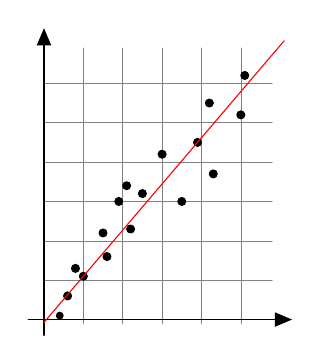
\begin{tikzpicture}[line cap=round,line join=round,>=triangle 45, domain=-.52:7, scale=1]
\tikzset{
    ultra thin/.style= {line width=0.1pt},
    very thin/.style=  {line width=0.2pt},
    thin/.style=       {line width=0.4pt},% thin is the default
    semithick/.style=  {line width=0.6pt},
    thick/.style=      {line width=0.8pt},
    very thick/.style= {line width=1.2pt},
    ultra thick/.style={line width=1.6pt}
}
%% Grid, axis and cliping of the figure
\draw[step=.5,help lines, very thin, color=gray] (0,-0.05) grid (2.9,3.45);
\draw[->] (-.2,0) -- (3.15,0); 
\draw[->] (0,-.2) -- (0,3.7);

\fill [black] (.2,.05) circle (0.05);
\draw [fill=black] (0.3,0.3) circle (0.05);
\draw [fill=black] (0.5,0.55) circle (0.05);
\draw [fill=black] (0.4,0.65) circle (0.05);
\draw [fill=black] (0.75,1.1) circle (0.05);
\draw [fill=black] (1.1,1.15) circle (0.05);
\draw [fill=black] (0.95,1.5) circle (0.05);
\draw [fill=black] (0.8,0.8) circle (0.05);
\draw [fill=black] (1.75,1.5) circle (0.05);
\draw [fill=black] (1.05,1.7) circle (0.05);
\draw [fill=black] (1.25,1.6) circle (0.05);
\draw [fill=black] (1.5,2.1) circle (0.05);
\draw [fill=black] (2.15,1.85) circle (0.05);
\draw [fill=black] (1.95,2.25) circle (0.05);
\draw [fill=black] (2.1,2.75) circle (0.05);
\draw [fill=black] (2.5,2.6) circle (0.05);
\draw [fill=black] (2.55,3.1) circle (0.05);

\draw [red] (0,-0.0362) -- (3.05,3.54);

\end{tikzpicture}

\end{document}